\documentclass[8pt]{article}

\usepackage{amsmath, amssymb, amsfonts}
\usepackage{graphicx}

\usepackage{hyperref}
\usepackage[margin=1in]{geometry}
\usepackage{fancyhdr}
\usepackage{parskip}
\usepackage{titlesec}
\usepackage{setspace}

\title{CAB320 - Artificial Intelligence Study Notes}
\author{Jaden Ussher}
\date{Last modified on 2022/03/02}

% Custom header and footer
\pagestyle{fancy}
\fancyhf{}
\fancyhead[L]{CAB320 Artificial Intelligence}
\fancyhead[R]{Study Notes}
\fancyfoot[C]{\thepage}

% Title formatting
\titleformat{\section}{\large\bfseries}{\thesection}{1em}{}
\titleformat{\subsection}{\normalsize\bfseries}{\thesubsection}{1em}{}
\titleformat{\subsubsection}{\normalsize\itshape}{\thesubsubsection}{1em}{}

% Adjust line spacing
\singlespacing

\begin{document}

\maketitle
\small
\newpage

\tableofcontents

\newpage
\section{Week 2 - Discrete Math Tools}
\subsection{Key Discrete Math Concepts for AI}
\begin{itemize}
    \item Recurrence relations and recursive functions
    \item Graphs and trees
    \begin{itemize}
        \item Data structure, abstraction, object-oriented programming
    \end{itemize}
    \item Graph properties
    \begin{itemize}
        \item Directedness, paths, connectivity, connected components, cycles, roots, sinks
    \end{itemize}
    \item Dijkstra's algorithm
    \begin{itemize}
        \item Computation of the shortest paths from a source to all other vertices
    \end{itemize}
\end{itemize}

\subsection{Graphs and Their Importance in AI}
\begin{figure}[h]
    \centering
    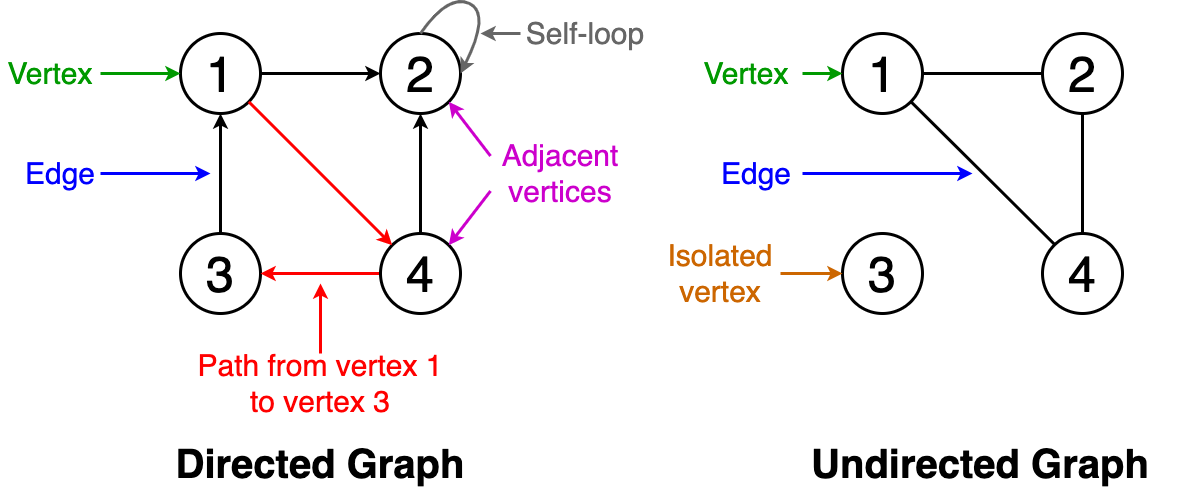
\includegraphics[width=0.5\linewidth]{images/1_xpy7aax3dIU12HVrGd_siQ.png}
    \caption{Graph Basics}
    \label{fig:enter-label}
\end{figure}

\begin{itemize}
    \item A graph \( G \) is a pair \( (V, E) \) where \( V \) is a set of vertices and \( E \) is a set of pairs of vertices called edges.
    \item Graphs do not need a visual representation to exist.
    \item Directed graphs (digraphs) have ordered edges, called arcs.
    \item Vertices are also known as nodes.
    \item In AI, graphs are used for:
    \begin{itemize}
        \item Planning problems: Finding a “good” sequence of actions can be reduced to finding a “good” path in an associated state graph.
        \item Knowledge representation: Social networks, scene representation, protein folding, etc.
    \end{itemize}
\end{itemize}

\subsection{Graph Representations}
\subsubsection{Adjacency Matrix}
\begin{itemize}
    \item For undirected graphs: A symmetric matrix where \( A[i][j] = 1 \) if there is an edge between vertices \( i \) and \( j \), otherwise \( 0 \).
    \item For directed graphs: \( A[i][j] = 1 \) if there is an arc from \( i \) to \( j \).
\end{itemize}

\subsubsection{Vertex-Arc Incidence Matrix}
\begin{itemize}
    \item Represents the incidence of vertices and arcs.
\end{itemize}

\subsubsection{Adjacency List}
\begin{itemize}
    \item Use dictionaries in Python where keys are vertices and values are lists of neighbors.
    \item Efficient for sparse graphs.
\end{itemize}

\subsection{Graph Properties}
\begin{itemize}
    \item Directedness: Graphs can be directed or undirected.
    \item Paths and connectivity:
    \begin{itemize}
        \item A path is a sequence of vertices connected by edges.
        \item Connectivity determines if there is a path between every pair of vertices.
        \item A connected component is a maximal connected subgraph.
    \end{itemize}
    \item Cycles: A path that starts and ends at the same vertex without repeating any edge or vertex.
    \item In-degree and Out-degree:
    \begin{itemize}
        \item In-degree: Number of incoming arcs to a vertex.
        \item Out-degree: Number of outgoing arcs from a vertex.
    \end{itemize}
\end{itemize}

\subsection{Special Graphs}
\subsubsection{Clique}
\begin{itemize}
    \item A clique is a subset of vertices such that every two distinct vertices are adjacent.
    \item Maximal clique: A clique that cannot be extended by including one more adjacent vertex.
\end{itemize}

\subsubsection{Interval Graph}
\begin{itemize}
    \item Vertices represent intervals, and there is an edge between two vertices if their corresponding intervals intersect.
    \item Always contains a vertex whose neighbors form a clique.
\end{itemize}

\subsection{Trees}
\begin{itemize}
    \item A tree is a connected, acyclic undirected graph. Equivalent conditions for trees:
    \begin{itemize}
        \item Connected and acyclic.
        \item Adding any edge creates a cycle.
        \item Removing any edge disconnects the graph.
        \item Unique simple path between any two vertices.
    \end{itemize}
\end{itemize}
\newpage
\subsection{Dijkstra's Algorithm}
\begin{itemize}
    \item Purpose: Find shortest paths from a source vertex to all other vertices in a weighted graph.
    \item Method:
    \begin{itemize}
        \item Initialize distances from the source to all vertices as infinity except the source itself, which is zero.
        \item Use a priority queue to repeatedly extract the vertex with the minimum distance.
        \item Update the distances of the adjacent vertices.
    \end{itemize}
\end{itemize}

\subsubsection*{Example 1}
\begin{figure}[h]
    \centering
    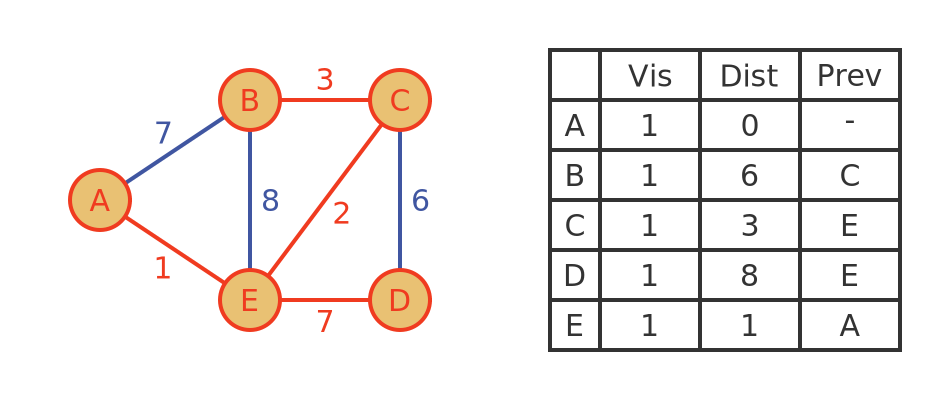
\includegraphics[width=0.5\linewidth]{images/algorithm-5.png}
    \caption{Dijkstra's Algorithm Visual Example}
    \label{fig:enter-label}
\end{figure}


\subsubsection*{Example 2}

\begin{verbatim}
Graph: (V, E) with weights
    V = {A, B, C, D}
    E = {(A, B, 1), (A, C, 4), (B, C, 2), (B, D, 5), (C, D, 1)}
Steps:
1. Initialize distances: dist[A]=0, dist[B]=∞, dist[C]=∞, dist[D]=∞
2. Extract A: dist[A]=0
    Update dist[B]=1, dist[C]=4
3. Extract B: dist[B]=1
    Update dist[C]=3, dist[D]=6
4. Extract C: dist[C]=3
    Update dist[D]=4
5. Extract D: dist[D]=4
Result: Shortest paths from A
    A -> B -> C -> D with distances 0, 1, 3, 4 respectively.
\end{verbatim}

\subsection*{Correctness of Dijkstra's Algorithm}
\begin{itemize}
    \item \textbf{Invariant Hypothesis}:
    \begin{itemize}
        \item For each vertex \( v \), \( \text{dist}[v] \) is an upper bound of the cost of a cheapest path from the source to \( v \).
        \item If \( v \) has been removed from the priority queue, \( \text{dist}[v] \) is the cost of the cheapest path.
    \end{itemize}
    \item Proof by induction on the size of \( V - L \) (where \( L \) is the set of unfinalized vertices).
    \item \textbf{Lemma}: If \( T \) is the tree of finalized vertices, any non-finalized vertex \( a \) adjacent to \( T \) has the cheapest path via its parent.
    \item \textbf{Contradiction}:
    \begin{itemize}
        \item If there is a strictly cheaper path, it would imply incorrect extraction order, violating the algorithm's logic.
    \end{itemize}
\end{itemize}

\section{Week 3 - Intelligence Agents \& Uniformed Search}
\subsection{Intelligence Agents}
\subsection{Key Concepts}
\subsubsection{Agents and Environments}
\begin{itemize}
    \item Agents include humans, robots, softbots, thermostats, etc.
    \item The agent function maps from percept histories to actions.
    \item Agents interact with environments through sensors and actuators.
\end{itemize}

\subsubsection{Vacuum-Cleaner World}
\begin{itemize}
    \item Percepts: Location and contents, e.g., [A, Dirty].
    \item Actions: Left, Right, Suck, NoOp.
    \item Example: A vacuum-cleaner agent must decide its actions based on its current percept.
\end{itemize}

\subsubsection{Rationality}
\begin{itemize}
    \item A rational agent chooses any action that maximizes the expected value of the performance measure given the percept sequence to date.
    \item Rationality maximizes expected outcome while perfection maximizes actual outcome.
    \item Rational does not mean omniscient or perfect.
\end{itemize}

\subsubsection{P.E.A.S. Framework}
\begin{itemize}
    \item To design a rational agent, we must specify the task environment, which consists of:
    \begin{itemize}
        \item Performance measure
        \item Environment
        \item Actuators
        \item Sensors
    \end{itemize}
    \item Examples:
    \begin{itemize}
        \item Automated taxi: Safety, streets, steering, video.
        \item Internet shopping agent: Price, WWW sites, display, HTML pages.
        \item Part-picking robot: Percentage of parts in correct bins, conveyor belt, jointed arm, camera.
    \end{itemize}
\end{itemize}

\subsubsection{Environment Types}
\begin{itemize}
    \item Deterministic vs. stochastic: Is the next state perfectly predictable?
    \item Static vs. dynamic: Does the environment change while the agent deliberates?
    \item Fully vs. partially observable: Does the agent have access to all relevant information?
    \item Single-agent vs. multi-agent: Are there other agents in the environment?
    \item Known vs. unknown: Does the agent understand the laws governing the environment?
    \item Episodic vs. sequential: Are past actions relevant to the current decision?
    \item Discrete vs. continuous: Are states and time intervals fixed or continuous?
\end{itemize}

\subsubsection{Agent Types}
\begin{itemize}
    \item Simple reflex agents: Choose actions based on current percept.
    \item Reflex agents with state: Have memory or a model of the world’s current state.
    \item Goal-based agents: Act to achieve specific goals.
    \item Utility-based agents: Maximize a utility function to measure performance.
    \item Learning agents: Improve their performance over time.
\end{itemize}

\subsubsection{Examples of Agent Types}
\begin{itemize}
    \item Reflex Agents: Edge following robot.
    \item Model-Based Reflex Agent: Vacuum robot that counts the number of cells cleaned.
    \item Model-Based Goal-Based Agent: Sokoban agent.
    \item Model-Based Utility-Based Agent: Pacman player.
    \item General Learning Agent: Self-balancing robot.
\end{itemize}

\newpage
\subsection{Uniformed Search}
\subsubsection{Planning Agents}
\begin{itemize}
    \item Planning agents ask "what if" and make decisions based on hypothesized consequences of actions.
    \item They must have a model of how the world evolves in response to actions.
    \item Formulation of a goal and consideration of how the world would be is essential.
    \item Distinguish between optimal vs. complete planning and planning vs. re-planning.
\end{itemize}

\subsection{State Types}
Different types of states in planning and search problems are considered.

\subsection{Search Problems}
A search problem consists of:
\begin{itemize}
    \item A state space.
    \item A successor function (with actions and costs).
    \item A start state and a goal test.
\end{itemize}
A solution is a sequence of actions (a plan) that transforms the start state to a goal state.

\subsection{Example Problems}
\begin{itemize}
    \item Romania: Finding paths between cities.
    \item Vacuum world: A simple robotic agent cleaning a room.
    \item The 8-puzzle: Sliding puzzle game.
    \item The 8-queens problem: Placing 8 queens on a chessboard without threatening each other.
    \item Robotic assembly: Planning the sequence of actions for assembling parts.
\end{itemize}

\subsection{Tree Search Algorithms}
Tree search algorithms explore possible sequences of actions to find a solution.

\subsection{Uninformed Search Strategies}
Uninformed search strategies are methods that search the state space without any domain-specific knowledge. These include:
\begin{itemize}
    \item Breadth-First Search (BFS)
    \item Uniform-Cost Search
    \item Depth-First Search (DFS)
    \item Depth-Limited Search
    \item Iterative Deepening Search
\end{itemize}

\newpage
\subsubsection{Breadth-First Search (BFS)}
\begin{itemize}
    \item Explores all nodes at the present depth level before moving on to nodes at the next depth level.
    \item Initial frontier: \{A\}
    \item Frontier after expanding A: \{B, C\}
    \item Frontier after expanding B: \{C, D, E\}
    \item Frontier after expanding C: \{D, E, F, G\}
\end{itemize}
Properties: Complete and optimal for unweighted graphs, but has high memory requirements.

\begin{figure}[!h]
    \centering
    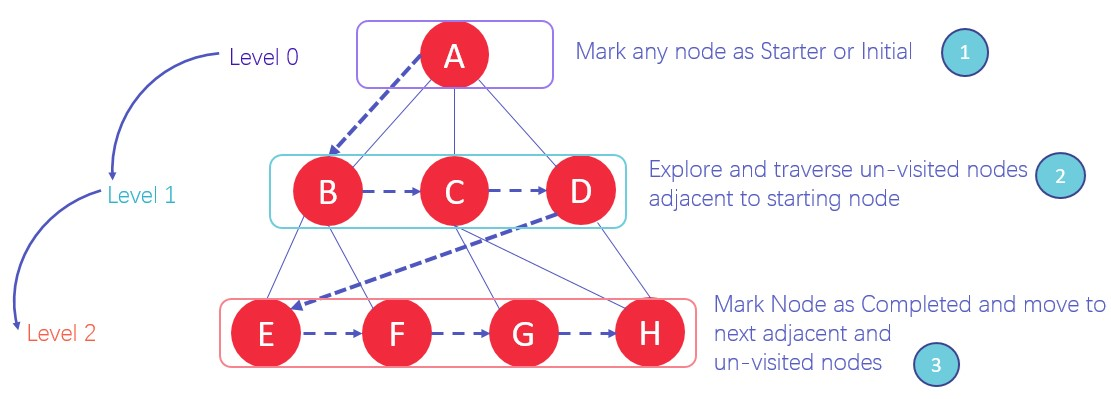
\includegraphics[width=0.5\linewidth]{images/020820_0543_BreadthFirs1ropped.jpg}
    \caption{BFS Algorithm}
    \label{fig:enter-label}
\end{figure}

\subsubsection{Uniform-Cost Search}
\begin{itemize}
    \item Expands the least-cost unexpanded node.
    \item Similar to Dijkstra's algorithm for shortest paths.
\end{itemize}

\begin{figure}[!h]
    \centering
    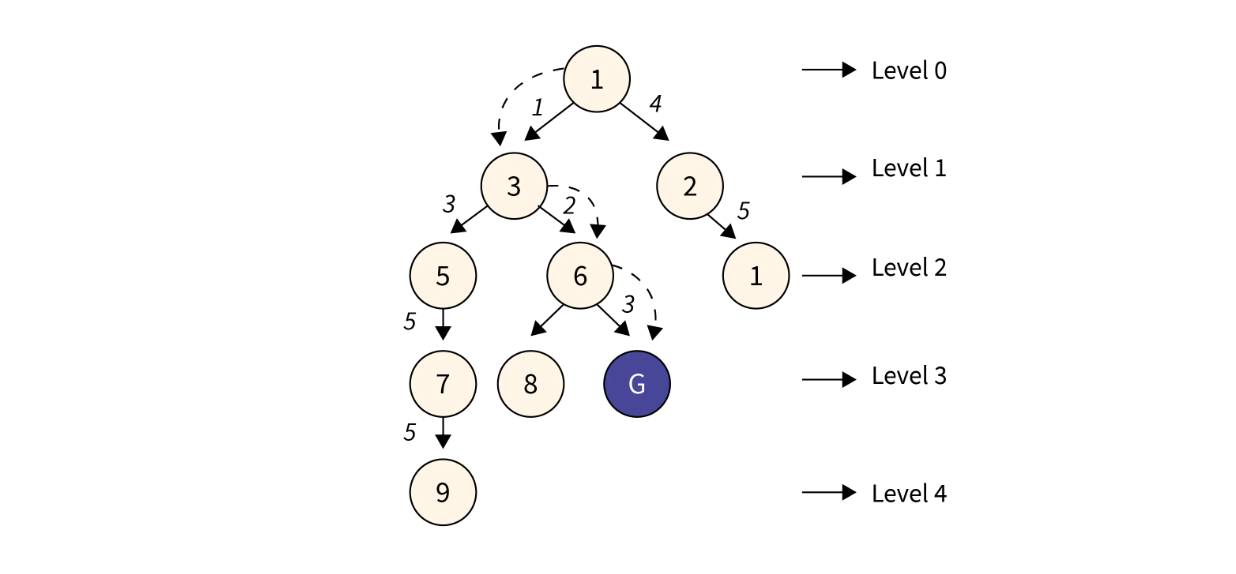
\includegraphics[width=0.5\linewidth]{images/uniform search.PNG}
    \caption{Uniform Cost Search Algorithm}
    \label{fig:enter-label}
\end{figure}

\subsubsection{Depth-First Search (DFS)}
\begin{itemize}
    \item Explores as far as possible along each branch before backtracking.
    \item Initial frontier: \{A\}
    \item Frontier after expanding A: \{B, C\}
    \item Frontier after expanding C: \{B, F, G\}
    \item Frontier after expanding G: \{B, F, N, O\}
\end{itemize}
Properties: May get stuck in infinite loops, not guaranteed to find the shortest path.

\begin{figure}[!h]
    \centering
    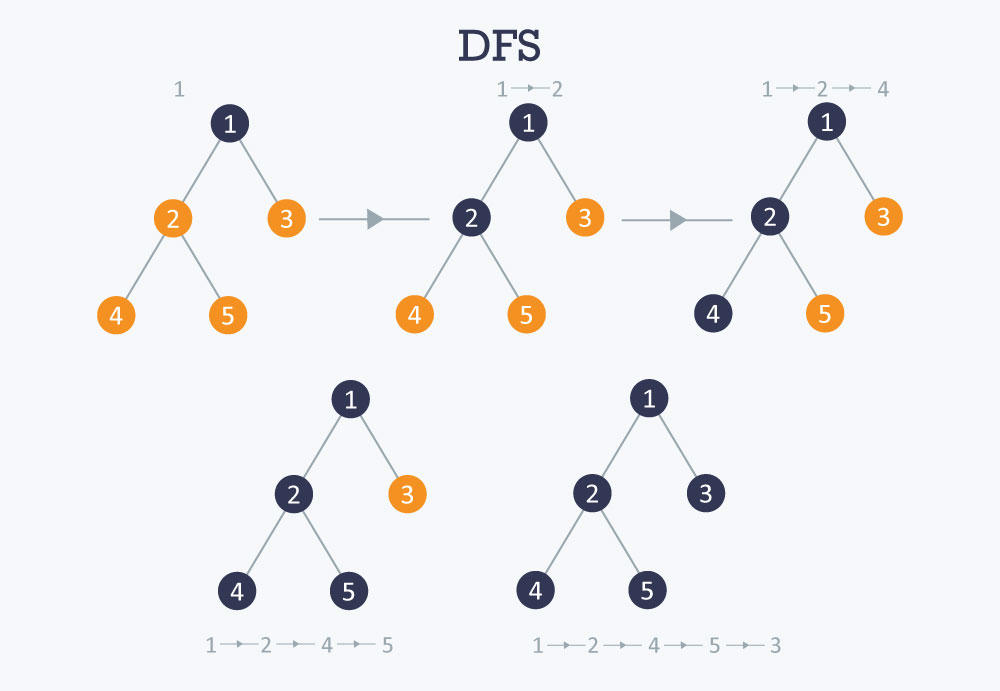
\includegraphics[width=0.5\linewidth]{images/DFS.jpg}
    \caption{Depth First Search Algorithm}
    \label{fig:enter-label}
\end{figure}

\newpage
\subsubsection{Depth-Limited Search}
\begin{itemize}
    \item Depth-first search with a limit on the depth.
    \item Useful for infinite depth or large search spaces.
\end{itemize}

\begin{figure}[!h]
    \centering
    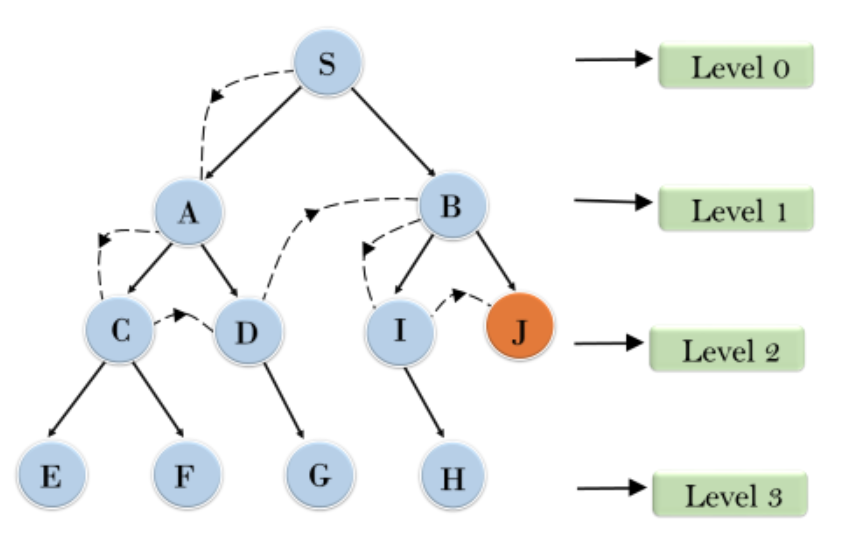
\includegraphics[width=0.5\linewidth]{images/dls.PNG}
    \caption{Depth Limited Search}
    \label{fig:enter-label}
\end{figure}

\subsubsection{Iterative Deepening Search}
\begin{itemize}
    \item Combines the benefits of BFS and DFS.
    \item Repeatedly applies DFS with increasing depth limits.
    \item Level 0: \{A\}
    \item Level 1: \{B, C\}
    \item Level 2: \{D, E, F, G\}
\end{itemize}
Properties: Complete and optimal like BFS, but with lower memory requirements.
\newpage
\subsection{Implementation Considerations}
\subsection*{States vs. Nodes}
\begin{itemize}
    \item States represent physical configurations.
    \item Nodes represent states with additional information, such as parent nodes, actions, and path costs.
\end{itemize}

\subsubsection{General Tree Search Algorithm}
The general tree search algorithm explores nodes in a tree structure, using different strategies to manage the frontier.

\subsubsection{Search Strategies}
Different strategies impact the efficiency and effectiveness of finding a solution.

\subsubsection{Graph Search}
\begin{itemize}
    \item Avoids expanding the same state multiple times.
    \item Maintains a frontier to explore and a set of explored nodes.
\end{itemize}
Example: Uniform-cost search on a subgraph of the Romania map.

\subsubsection{Bidirectional Search}
\begin{itemize}
    \item Searches from both the start and goal states simultaneously.
    \item Can significantly reduce search time.
\end{itemize}

\newpage
\section{Wek 4 - A* Search and Search Heuristics}
\subsection{A* Search Algorithm}
\begin{itemize}
    \item Combines the strengths of Uniform Cost Search (UCS) and Greedy Search.
    \item Uses both path cost \(g(n)\) and heuristic cost \(h(n)\).
    \item Expands nodes based on the evaluation function \(f(n) = g(n) + h(n)\).
\end{itemize}

\subsubsection{Key Properties of A*}
\begin{itemize}
    \item \textbf{Completeness:} A* is complete if the branching factor is finite and the cost of every step is greater than a positive constant.
    \item \textbf{Optimality:} A* is optimal if the heuristic used is admissible (i.e., it never overestimates the true cost).
    \item \textbf{Admissible Heuristics:} Heuristic \(h(n)\) is admissible if \(0 \leq h(n) \leq h^*(n)\), where \(h^*(n)\) is the true cost to reach the goal from node \(n\).
    \item \textbf{Efficiency:} The efficiency of A* depends on the quality of the heuristic function. Better heuristics result in fewer nodes being expanded.
\end{itemize}

\subsubsection{Example: A* Search for Pathfinding}
\begin{itemize}
    \item Consider finding a path in a grid from a start node \(S\) to a goal node \(G\).
    \item \textbf{Path Cost \(g(n)\):} The cost to reach node \(n\) from the start node \(S\).
    \item \textbf{Heuristic Cost \(h(n)\):} An estimate of the cost to reach the goal node \(G\) from node \(n\). For instance, Manhattan distance or Euclidean distance.
    \item \textbf{Evaluation Function \(f(n)\):} \(f(n) = g(n) + h(n)\).
    \item A* search explores nodes in order of increasing \(f(n)\) values.
\end{itemize}

\subsubsection{Algorithm Steps}
\begin{enumerate}
    \item Initialize the open list with the start node \(S\).
    \item Initialize the closed list as empty.
    \item Loop until the open list is empty or the goal node is found:
    \begin{enumerate}
        \item Remove the node \(n\) with the lowest \(f(n)\) from the open list.
        \item If \(n\) is the goal node \(G\), reconstruct the path from \(S\) to \(G\).
        \item Generate successors of node \(n\).
        \item For each successor:
        \begin{itemize}
            \item Calculate \(g(\text{successor})\) and \(f(\text{successor})\).
            \item If the successor is not in the open list or has a lower \(f\) value, add it to the open list.
        \end{itemize}
        \item Add node \(n\) to the closed list.
    \end{enumerate}
\end{enumerate}

\subsection{Search Heuristics}
\begin{itemize}
    \item \textbf{Definition:} A heuristic is a function that estimates the cost to reach the goal from a given state.
    \item \textbf{Purpose:} Heuristics guide the search process, making it more efficient by prioritizing nodes that are more likely to lead to the goal.
\end{itemize}

\subsubsection{Properties of Heuristics}
\begin{itemize}
    \item \textbf{Admissibility:} A heuristic is admissible if it never overestimates the cost to reach the goal.
    \item \textbf{Consistency (Monotonicity):} A heuristic is consistent if, for every node \(n\) and every successor \(n'\) of \(n\), the estimated cost to reach the goal from \(n\) is no greater than the cost of getting to \(n'\) plus the estimated cost from \(n'\) to the goal.
\end{itemize}

\subsubsection{Examples of Heuristics}
\begin{itemize}
    \item \textbf{Manhattan Distance:} Used for grid-based pathfinding where movement is restricted to horizontal and vertical steps.
    \[
    h(n) = |x_1 - x_2| + |y_1 - y_2|
    \]
    \item \textbf{Euclidean Distance:} Used for grid-based pathfinding where movement can be in any direction.
    \[
    h(n) = \sqrt{(x_1 - x_2)^2 + (y_1 - y_2)^2}
    \]
    \item \textbf{Example in Pathfinding:} 
    \begin{itemize}
        \item In a grid, if the current node is at \((2, 3)\) and the goal node is at \((5, 7)\):
        \item Manhattan distance heuristic: \(h(n) = |2 - 5| + |3 - 7| = 3 + 4 = 7\).
        \item Euclidean distance heuristic: \(h(n) = \sqrt{(2 - 5)^2 + (3 - 7)^2} = \sqrt{9 + 16} = \sqrt{25} = 5\).
    \end{itemize}
\end{itemize}

\subsubsection{Heuristics for Specific Problems}
\begin{itemize}
    \item \textbf{Sliding Puzzle:} Number of tiles out of place, total Manhattan distance of tiles from their goal positions.
    \item \textbf{Traveling Salesperson Problem (TSP):} Minimum spanning tree (MST) heuristic, nearest neighbor heuristic.
\end{itemize}



\end{document}
